%!TEX root = ../main.tex
%---------------------------------------------------------------------------------------------------
\subsection{Data}\label{Appendix data}\FloatBarrier
%---------------------------------------------------------------------------------------------------
We use the same data as \citetAppndx{Keane.1997}, who derive their sample from the National Longitudinal Survey of Youth 1979 (NLSY79) \citepAppndx{NLSY.2019}. The NLSY79 is a nationally representative sample of young men and women living in the United States in 1979 and born between 1957 and 1964. Individuals were followed from 1979 onwards and repeatedly interviewed about their educational decisions and labor market experiences. Based on this information, individuals are assigned to either working in one of three occupations, attending school, or simply staying at home. The decision period is represented by the school year. The sample is restricted to white men, who turned 16 between 1977 and 1981, and it uses information collected between 1979 and 1987. Thus, the individuals in the sample range in age between 16 and 26 years old.\\

\noindent Figure \ref{Sample size} shows the sample size by age. While the sample initially consists of 1,373 16-year-olds, this value drops to 256, once the sampled individuals reach the age of 26 due to sample attrition, missing data, and the short observation period. Overall, the final sample consists of 12,359 person-period observations.\\

\begin{figure}[ht!]\centering
\scalebox{0.35}{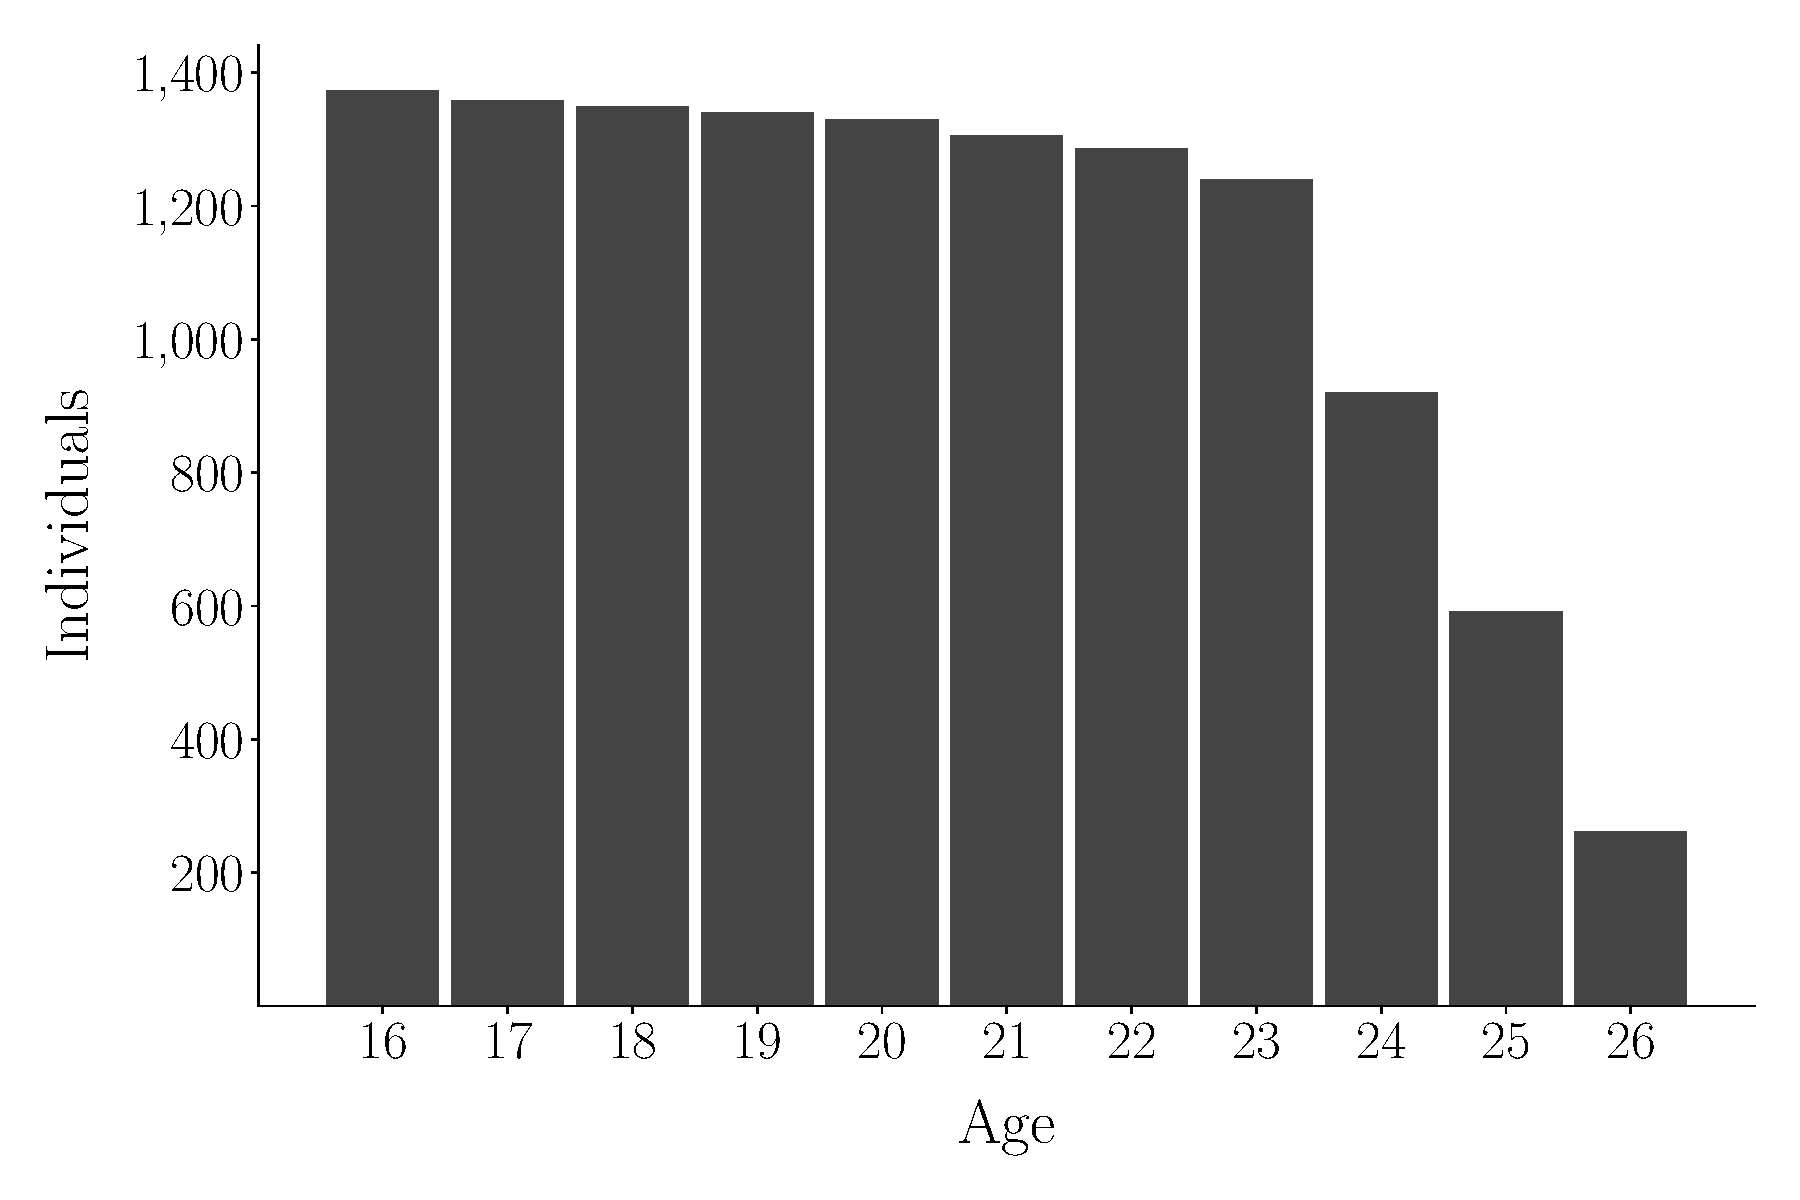
\includegraphics{fig-sample-size-bw}}
\caption{Sample size}\label{Sample size}
\end{figure}\FloatBarrier

\noindent Figure \ref{Initial schooling} shows the distribution of initial schooling among individuals at the time they enter the model. The majority of individuals enter the model with ten years of schooling, while about a quarter of the sample has less than ten years of schooling. About $7.5\%$ of individuals already attended school for 11 years.\\

\begin{figure}[ht!]\centering
\scalebox{0.35}{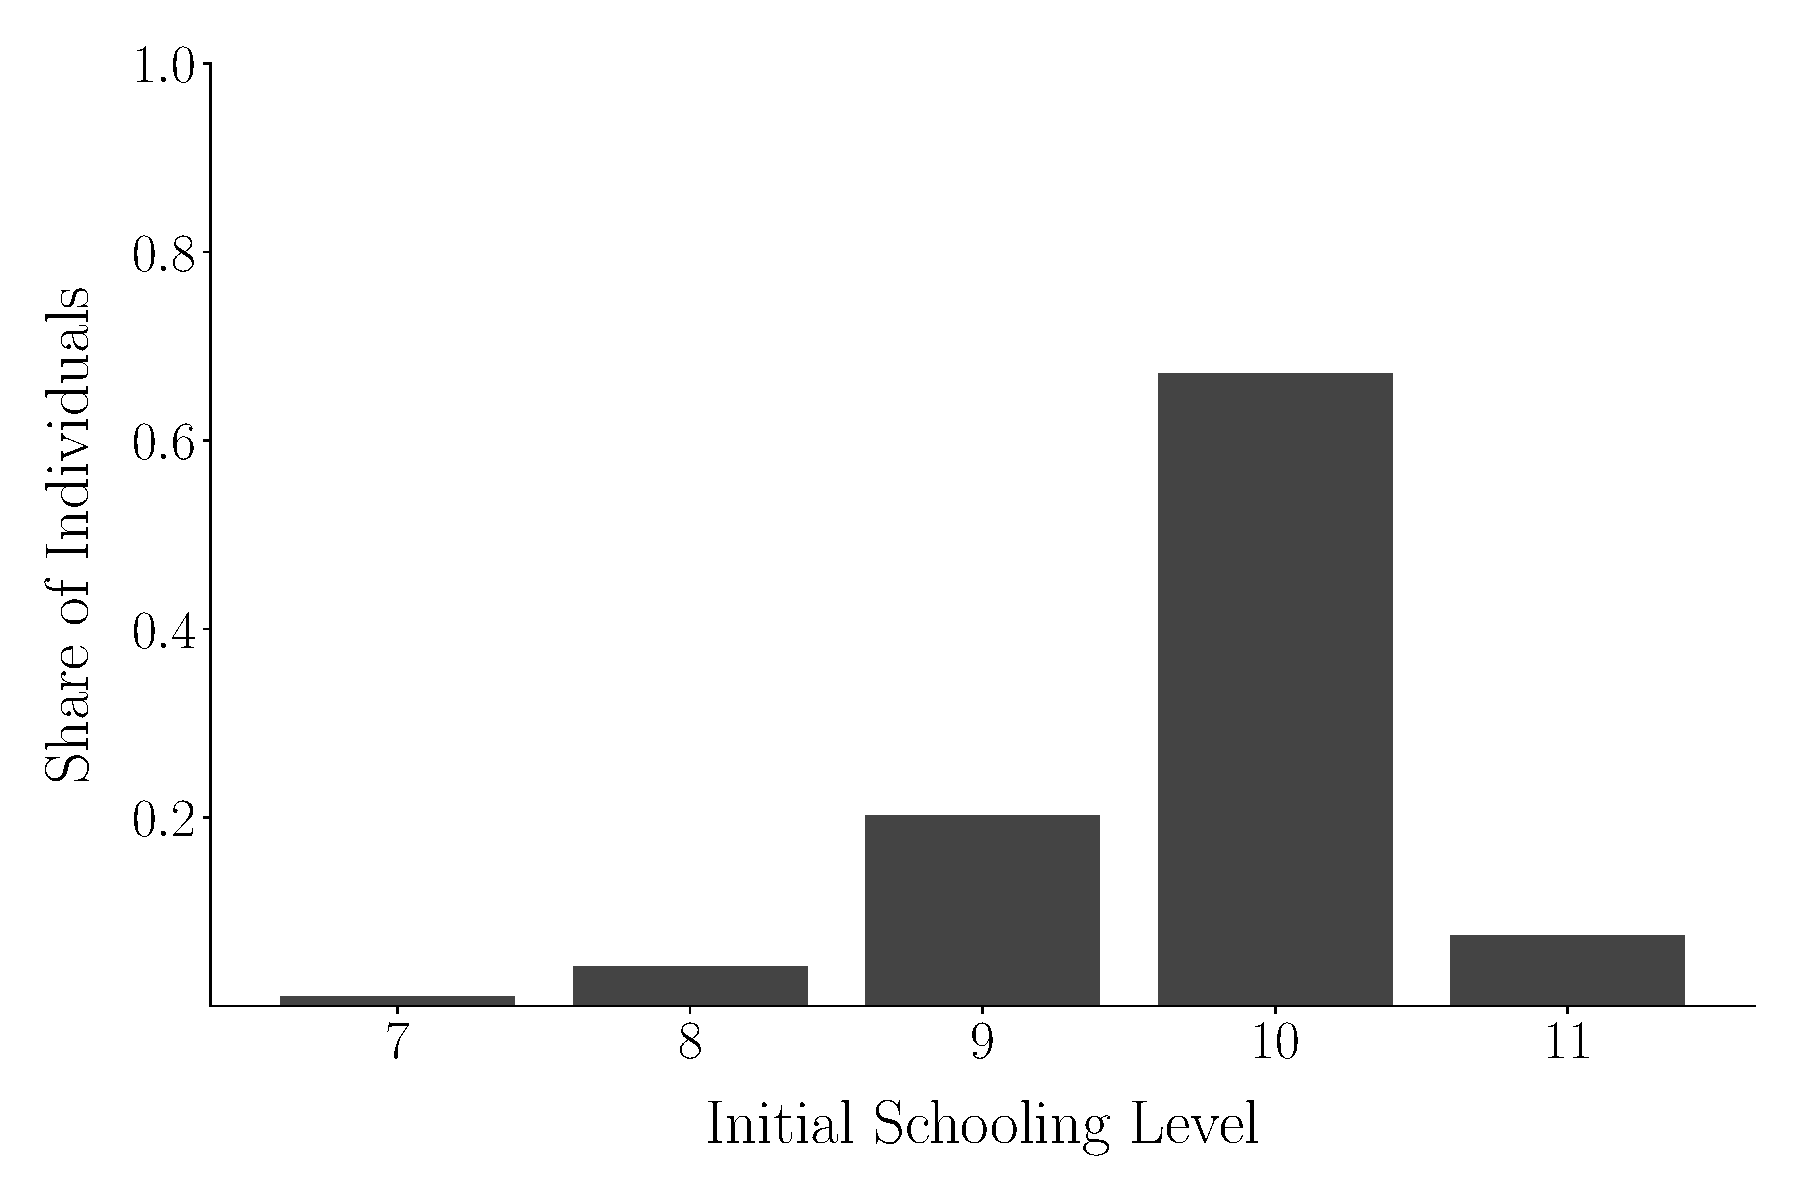
\includegraphics{fig-initial-schooling-bw}}
\caption{Initial schooling}\label{Initial schooling}
\end{figure}\FloatBarrier

\noindent Figure \ref{Average choices by initial schooling} shows heterogeneity of choices by the level of initial schooling. Individuals who enter the model with only seven years of schooling spend an additional 0.65 years in school after age 16. Consequently, they spend around four years at home. In the event that they are working, it is likely in a blue-collar occupation. When starting with ten years of schooling, then individuals add roughly another three years while in the model. This increase is about half a year more than individuals that start with eleven years.\\

\begin{figure}[ht!]\centering
\scalebox{0.35}{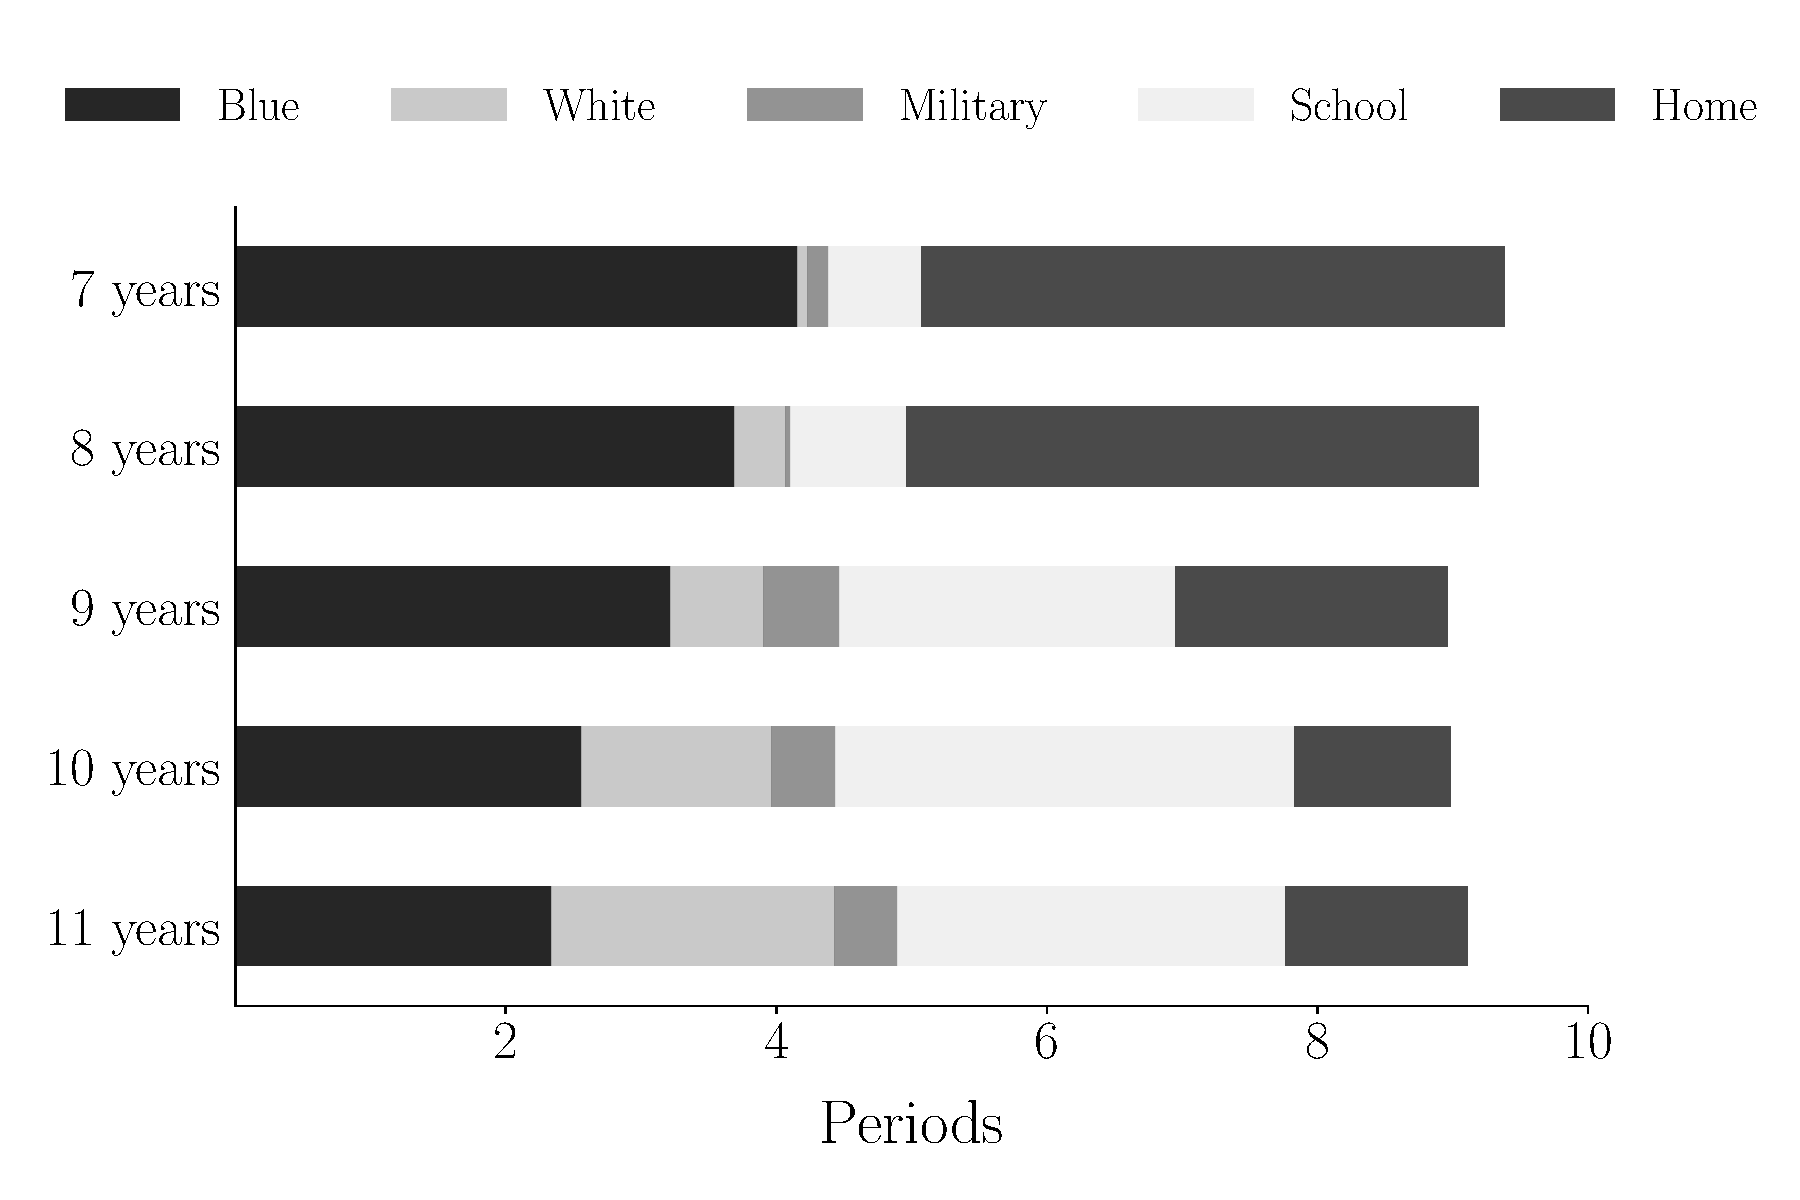
\includegraphics{fig-average-choices-by-initial-schooling-bw}}
\caption{Average choices by initial schooling}\label{Average choices by initial schooling}
\end{figure}\FloatBarrier

\noindent Figure \ref{Transition matrix} documents strong persistence in choices over time. For example, among those with a white-collar occupation in $t$, 67\% work in the same occupation in $t + 1$, while $20\%$ switch to a blue-collar job.\\

\begin{figure}[h]\centering
\scalebox{0.35}{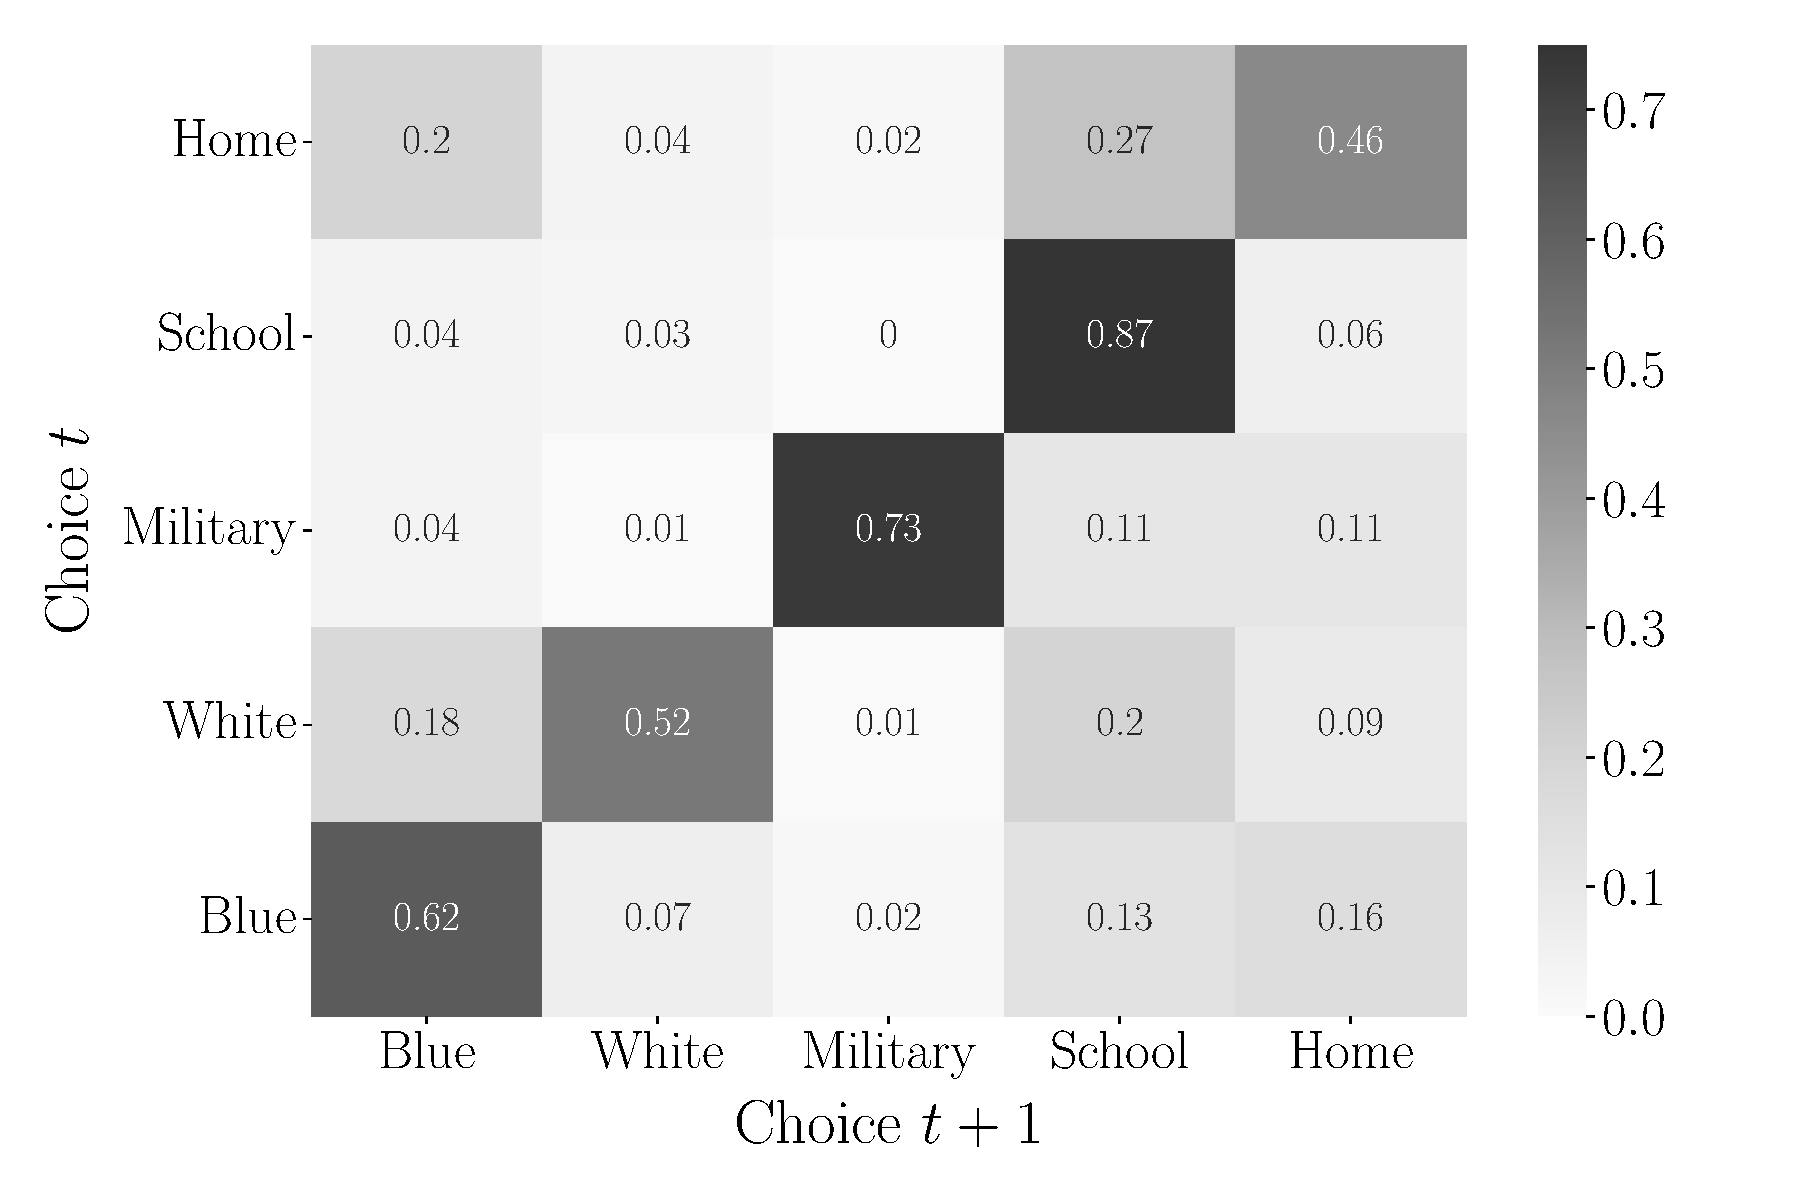
\includegraphics{fig-heatmap-transitionprobs-bw}}
\caption{Transition matrix}\label{Transition matrix}
\end{figure}\FloatBarrier
